% This is a LaTeX thesis template for Monash University.
% to be used with Rmarkdown
% This template was produced by Rob Hyndman
% Version: 6 September 2016

\documentclass{monashthesis}

%%%%%%%%%%%%%%%%%%%%%%%%%%%%%%%%%%%%%%%%%%%%%%%%%%%%%%%%%%%%%%%
% Add any LaTeX packages and other preamble here if required
%%%%%%%%%%%%%%%%%%%%%%%%%%%%%%%%%%%%%%%%%%%%%%%%%%%%%%%%%%%%%%%

\author{Nicholas S Spyrison}
\title{Dynamic visualization of high-dimensional data via low-dimension
projections and sectioning across 2D and 3D display devices}
\degrees{B.Sc. Statistics, Iowa State University}
\def\degreetitle{Doctor of Philosophy}
% Add subject and keywords below
\hypersetup{
     %pdfsubject={The Subject},
     %pdfkeywords={Some Keywords},
     pdfauthor={Nicholas S Spyrison},
     pdftitle={Dynamic visualization of high-dimensional data via low-dimension
projections and sectioning across 2D and 3D display devices},
     pdfproducer={Bookdown with LaTeX}
}


\bibliography{thesisrefs}

\begin{document}

\pagenumbering{roman}

\titlepage

{\setstretch{1.2}\sf\tighttoc\doublespacing}

\chapter{spinifex: manual control of dynamic linear projections of
high-dimensional
data}\label{spinifex-manual-control-of-dynamic-linear-projections-of-high-dimensional-data}

\section{Abstract}\label{abstract}

The class of dynamic linear projections that are collectively known as
`tours' provide a unique means of visualizing numeric multivariate data.
Tours are particularly useful for understanding the structure held
within multivariate data, and in association with techniques for
dimension reduction, supervised, and unsupervised classification. The
\emph{R} package \emph{tourr} offers a variety of path generators and
geometric displays for conducting tours. This paper discusses an
extension package, \emph{spinifex}, that adds support for the path
generation of manual tours and extends the display of tours to use with
the contemporary animation packages, \emph{plotly} and \emph{gganimate}.
Manual tours are used to explore the sensitivity of structure as the
contributions of a manipulation variable are changed. This particularly
useful after identifying a feature of interest.

Keywords: manual tour, guided tour, grand tour, projection pursuit, high
dimensional data, multivariate data, data visualization, statistical
graphics, data science.

\section{Introduction}\label{introduction}

A tour is a multivariate data analysis technique in which a sequence of
linear (orthogonal) projections are viewed as an animation while the
orientation of the projection basis is rotated across time. Each frame
of the sequence corresponds to a small change in the projection for a
smooth transition that perseveres continuity.

While there are numerous methods that generate tour paths, this research
focuses on the manual tour. The manual tour was described in
\textcite{cook_manual_1997} and allows a user to control the projection
coefficients of a select variable has in a 2D projection. The
manipulation of these coefficients allows the analyst to explore how
sensitive the projections structure is to these changes. This makes
manual tours particularly useful once a feature of interest has been
identified, for example, with the use of a guided tour
\autocite{cook_grand_1995}. The path of a guided tour is selected via
projection pursuit, the optimization of an index function on the
projection via a hill climbing algorithm. This allows guided tours to
identify interesting projection features rapidly given the relatively
large parameter-space. Once the given projection has been provided, it
is time to define the path of rotation.

Ideally the path would be intuitively user-generated from physical
movement, be it through mouse or motion capture. Unfortunately this type
of dynamic control has proven difficult to capture for in R. Because of
this manual tours were not implemented within \emph{tourr}. This
research allows for the consumption, but not the generation, of such
dynamic input. After the capture of an oblique user motion the rotation
needs to be applied to step 3 (rotation sequence) of the algorithm
discussed below. In the section below we stick with a radial rotation
where, \(\theta\), the angle of in-projection-plane rotation is held
constant.

Spinifex utilizes two new animation packages, \emph{plotly}
\autocite{sievert_plotly_2018} and \emph{gganimate}
\autocite{pedersen_gganimate:_2019}, to display tours, manual or other
saved tours. From a given projection, the user can choose which variable
to control, and the animation sequence is generated to remove the
variable from the projection, and then extend its contribution to be the
sole variable in one direction. This allows the viewer to assess the
change in structure induced in the projection by the variable's
contribution.

The paper is organized as follows. Section \ref{sec:algorithm} explains
the algorithm using a toy dataset. Section \ref{sec:display} discussed
the display of the animation after the path has been generated. Section
\ref{sec:application} illustrates how this can be used for sensitivity
analysis applied to contemporary high energy physics. The last section,
\ref{sec:discussion} summarizes the work and discusses future research.

\section{Algorithm}\label{sec:algorithm}

The section below discribes the algorithm for performing a 2D radial
manual tour:

\begin{enumerate}
\def\labelenumi{\arabic{enumi}.}
\tightlist
\item
  Provided with a 2D projection, choose a variable to explore. This is
  called the ``manip'' variable.
\item
  Create a 3D manipulation space, where the manip variable has the full
  contribution.
\item
  Generate a rotation sequence which increases the norm of the
  coefficient to 1 and zeros it.
\end{enumerate}

The steps are described in more detail below.

\subsection{Notation}\label{notation}

This section describes the notation used in the algorithm for a 2D
radial manual tour.

\begin{itemize}
  \item $\textbf{X}$, the data, an $n \times p$ numeric matrix to be embedded in two dimensions.
  \item $\textbf{B} = (B_1,~ B_2)$, any of orthonormal projection basis set, $p \times 2$ matrix, describing the projection from $p$ to two dimensions
  \item $\textbf{e}$, a zero column vector of length $p$ with the $k-$th element set to one, where $k$ is the number of the variable to manipulate.
  \item $\theta$, the angle of in-projection-plane rotation, for example, on the reference axes. 
  \item $\phi$, the angle of out-of-projection-plane rotation, coming into the manipulation space.
\end{itemize}

The algorithm primarily operates on the projection basis and utilizes
the data only when making a display. The projection space can be viewed
at any point in the process by pre-multiplying the data and ploting the
first 2 variables.

\subsection{Toy data set}\label{toy-data-set}

The flea data, originally from \textcite{lubischew_use_1962}, available
in the R package \emph{tourr} \autocite{wickham_tourr_2011} is used to
illustrate the algorithm. The data contains 74 observations across 6
variables, physical measurements of the flea beetles. Each observation
belonging to one of three species.

The data is defined. A basis set (ideally that views an interesting
feature) should to be provided to explore the sensitivity of the
variables to the structure. To indentify a projection containing an
interesting feature, apply a guided tour\autocite{cook_interactive_2007}
on the flea data. In a guided tour the projection sequence is selected
by optimizing an index via hill-climbing. In this case, the holes index
is selected. The holes index is maximized by when the projected
observations are furthest from the center. Figure \ref{fig:step0} shows
a locally optimized projection for this data. The left plot displays the
reference axes of the projection basis, a visual indication of the
magnitude and direction each variable contributed to the projections.
The right plot shows the projection of the data through the basis set
decribed by the reference axes (left). Data points are colored and given
point characters according to the species of the flea (the guided tour
was unsupervised with this information).

\begin{figure}

{\centering 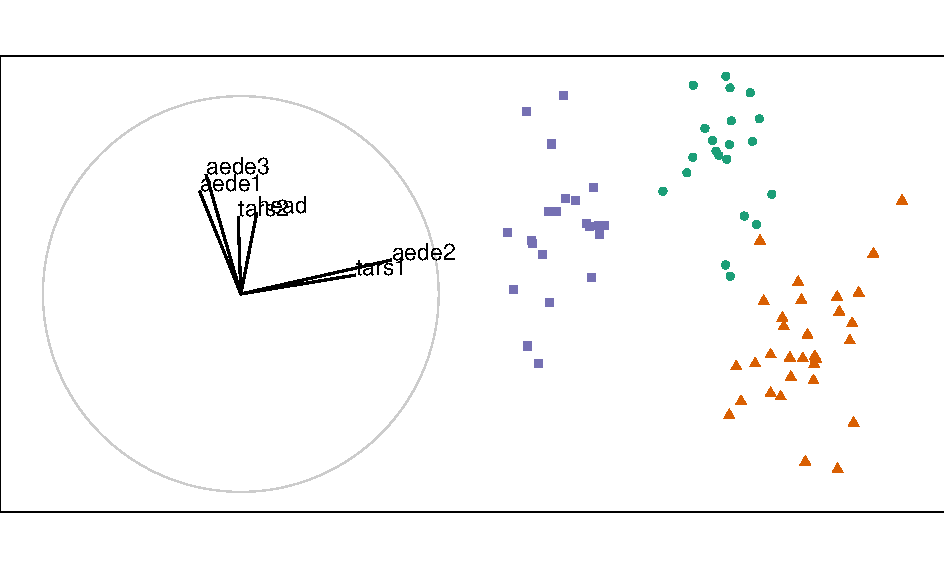
\includegraphics[width=0.95\linewidth,height=0.95\textheight]{confirmation_report_ns_files/figure-latex/step0-1} 

}

\caption{Basis reference axes (left) and projected data (right) of standardized flea data. Data points color and shape are mapped to beetle species. Basis identified by holes-index guided tour. The variables `aede2` and `tars1` contribute mostly orthogonal to the other variables. We'll select `aede2` as our manipulation variable to see how the structure of the projection changes as we rotate `aede2` into and out of the projection.}\label{fig:step0}
\end{figure}

Call \texttt{view\_basis()} on a basis to produce a \texttt{ggplot2}
graphic similar to \ref{fig:step0}. Projection space is always available
for display via the matrix multiplication
\(\textbf{X}_{[n,~p]} ~*~ \textbf{B}_{[p,~d]} ~=~ \textbf{P}_{[n,~d]}\).

\subsection{Step 1) Choose variable of
interest}\label{step-1-choose-variable-of-interest}

In figure \ref{fig:step0}, above, the contributions of the variables
\texttt{tars1} and \texttt{aede2} are mostly orthogonal to the
contributions of the other four variables. These two variables explain
the variation of the data between the purple and green species. We
select \texttt{aede2} as the manip var, the variable to be manipulated
as \texttt{aded2} typically has a larger contribution after the
optimizing the holes index. The question that will be explored in the
explanation of the algorithm is how important the variable
\texttt{aede2} is to the separation of the clusters.

\section{TODO: continue here.}\label{todo-continue-here.}

\subsection{Step 2 Create the manip
space}\label{step-2-create-the-manip-space}

Initialize a zero vector \(e\) of \(p\) elements. Because \texttt{aede2}
is the fifth variable in the data, set the \(k=5\)-th element to one
giving the manip var a full contribution in this dimension. Use the
Gram-Schmidt process to orthonormalize the zero vector onto the basis
yielding the 3D manipulation space.

\begin{align*}
  \textbf{e} &\leftarrow Orthonormalize_{GS}(\textbf{e}) \\
  &= \textbf{e} - \langle \textbf{e},\textbf{B}_1 \rangle \textbf{B}_1 - \langle \textbf{e}, \textbf{B}_2 \rangle \textbf{B}_2 \\
  \\
  \textbf{M}_{[p,~3]} &= (\textbf{B}_1,\textbf{B}_2,\textbf{e})
\end{align*}

Adding an extra dimension to our basis plane allows for the manipulation
of the specified variable. For example, lifting a piece of paper, rather
than manipulating on a table top. Orthonormalizing rescales the new
vector while leaving the first \(d\) variables identical to the basis.
An illustration of such can be seen below in figure \ref{fig:step2}.

\begin{figure}

{\centering 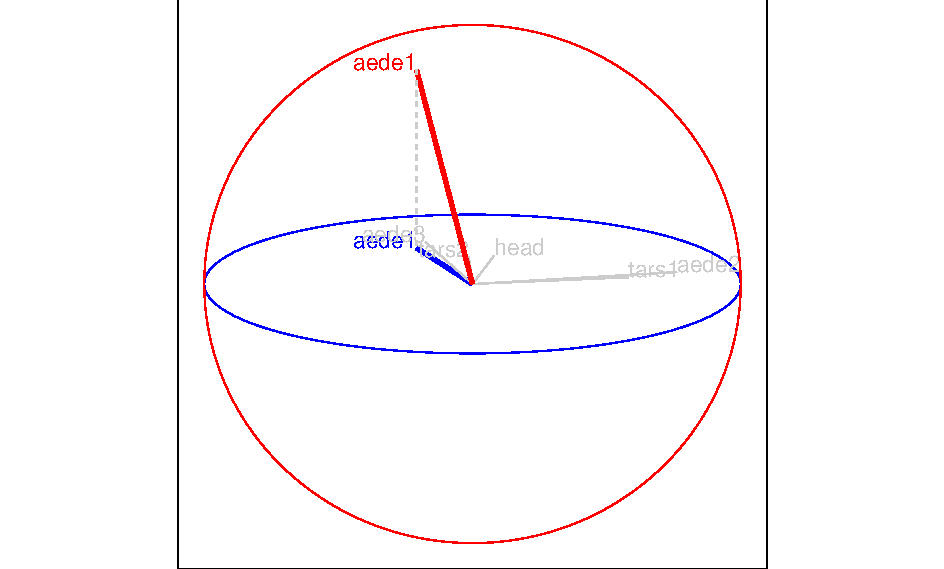
\includegraphics[width=1\linewidth]{confirmation_report_ns_files/figure-latex/step2-1} 

}

\caption{Manipulation space for controlling the contribution of aede2 of standardized flea data. Basis was identified by holes-index guided tour. The out of plane axis, in red, shows how the manipulation variable can be rotated, while other dimensions stay embedded within the basis plane.}\label{fig:step2}
\end{figure}

Imagine being able to grab hold of the red axis and rotate it changing
the projection onto the basis plane. This is what happens in a manual
tour. For a radial tour, fix \(\phi\), the angle within the blue plane,
and vary the \(\theta\), the angle between the red and blue lines. The
user controlling these angles changes the values of the coefficient the
manip variable and performs a constrained rotation on the remaining
variables.

\subsection{Step 3 Generate rotation}\label{step-3-generate-rotation}

Define a set of values for \(\phi_i\), the angle of out of the plane
rotation, orthogonal to the projection plane. This corresponds to the
angle between the red manipulation axis and the blue plane in figure
\ref{fig:step2}.

\textbf{For } \(i\) \textbf{in 1 to n\_slides:}

Post-multiply the manipulation space by a rotation matrix, producing,
\textbf{RM}, the rotated manip space.

\begin{align*}
  \textbf{RM}_{[p,~d+1,~i]}
  &= \textbf{M}_{[p,~d+1]} ~*~ \textbf{R}_{[d+1,~d+1]}
    ~~~~~~~~~~~~~~~~~~~~~~~~\text{For the $d=2$ case:} \\
  &= \begin{bmatrix}
    M_{1,~1} & \dots & M_{1,~d} & M_{1,~d+1} \\
    M_{2,~1} & \dots & M_{2,~d} & M_{2,~d+1} \\
    \vdots   & \ddots& \vdots   \\
    M_{p,~1} & \dots & M_{p,~d} & M_{p,~d+1}
  \end{bmatrix}_{[p,~d+1]}
    ~*~
  \begin{bmatrix}
    c_\theta^2 c_\phi s_\theta^2 &
    -c_\theta s_\theta (1 - c_\phi) &
    -c_\theta s_\phi \\
    -c_\theta s_\theta (1 - c_\phi) &
    s_\theta^2 c_\phi + c_\theta^2 &
    -s_\theta s_\phi \\
    c_\theta s_\phi &
    s_\theta s_\phi &
    c_\phi
  \end{bmatrix}_{[3,~3]}
\end{align*}

Where:

\begin{description}
  \item[$\theta$] is the angle that lies on the projection plane, the *XY*-scatterplot
  \item[$\phi$] is the angle orthogonal to the projection plane, in the *Z* direction relative to the *XY*-scatterplot
  \item[$c_\theta$] is the cosine of $\theta$
  \item[$c_\phi$]   is the cosine of $\phi$
  \item[$s_\theta$] is the sine of   $\theta$
  \item[$s_\phi$]   is the sine of   $\phi$
\end{description}

In application: compile the sequence of \(\phi_i\) and create an array
(or long table) for each rotated manipulation space. \(\phi\) is the
angle relative to the initial value of \(\phi\), we find the
transformation \(\phi_i\) - \(\phi_1\) useful to think about \(\phi\)
relative to the basis plane. If the manip variable doesn't move as
expected this is the first place to check.

\begin{Shaded}
\begin{Highlighting}[]
\ControlFlowTok{for}\NormalTok{ (phi }\ControlFlowTok{in} \KeywordTok{seq}\NormalTok{(seq_start, seq_end, phi_inc_sign)) \{}
\NormalTok{  slide <-}\StringTok{ }\NormalTok{slide }\OperatorTok{+}\StringTok{ }\DecValTok{1}
\NormalTok{  tour[,, slide] <-}\StringTok{ }\KeywordTok{rotate_manip_space}\NormalTok{(manip_space, theta, phi)[, }\DecValTok{1}\OperatorTok{:}\DecValTok{2}\NormalTok{]}
\NormalTok{\}}
\end{Highlighting}
\end{Shaded}

In figure \ref{fig:step3} we illustrate the sequence with 15 projected
bases and highlight the manip variable on top while showing the
corresponding projected data points on the bottom. A dynamic version of
this tour can be viewed online at
\url{https://nspyrison.netlify.com/thesis/flea_manualtour_mvar5/}, which
may take a moment to load. The format of this figure and linking to a
dynamic version will be used again in section \ref{sec:application}.









\begin{figure}

{\centering 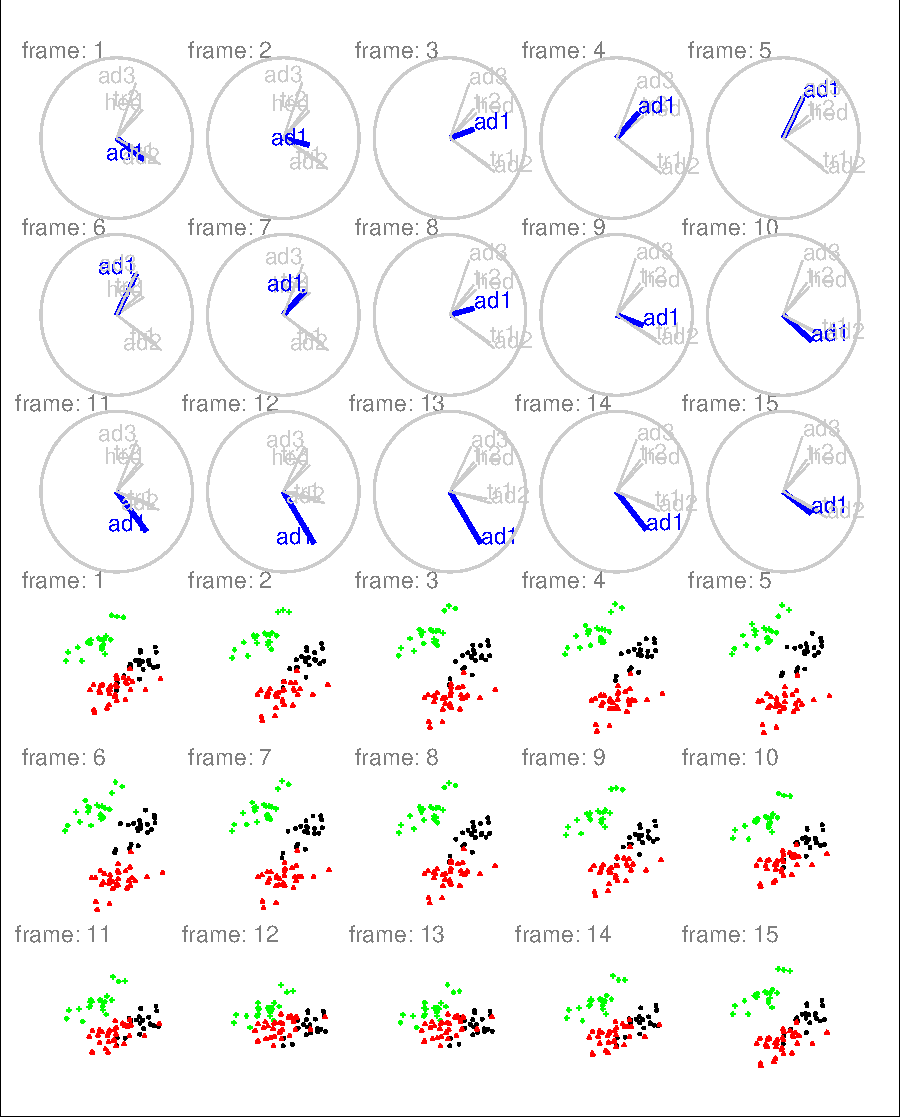
\includegraphics[width=6in,height=7.2in]{confirmation_report_ns_files/figure-latex/step3-1} 

}

\caption{Rotated manipulation spaces, a radial manual tour
controlling the contribution from \texttt{aded2} of standardized flea
data. The contribution of \texttt{aede2} extends from its initial
contribution to a full contribution to the projection before decreasing
to zero and then returning to its initial value. A dynamic version can
be viewed at
\url{https://nspyrison.netlify.com/thesis/flea_manualtour_mvar5/}.}\label{fig:step3}
\end{figure}

\section{Display projection sequence}\label{sec:display}

To get back to data-space pre-multiply each rotated manip space by the
data for the projection in data-space.

\begin{align}
  \textbf{P}_{[n,~d+1]}
    &= \textbf{X}_{[n,~p]} ~*~ \textbf{RM}_{[p,~d+1]} \\
    &=
      \begin{bmatrix}
          X_{1,~1} & \dots & X_{1,~p} \\
          X_{2,~1} & \dots & X_{2,~p} \\
          \vdots   & \vdots & \vdots  \\
          X_{n,~1} & \dots & X_{n,~p}
      \end{bmatrix}_{[n,~p]}
      ~*~
      \begin{bmatrix}
        RM_{1,~1} & RM_{1,~2} & RM_{1,~3} \\
        RM_{2,~1} & RM_{2,~2} & RM_{2,~3} \\
        \vdots     & \vdots     & \vdots     \\
        RM_{p,~1} & RM_{p,~2} & RM_{p,~3}
      \end{bmatrix}_{[p,~d+1]}
\end{align}

Plot the first 2 variables from each projection in sequence for an
\(XY\) scatterplot. The remaining variable is sometimes linked to a data
point aesthetic to produce depth cues used in conjunction with the
\(XY\) scatterplot.

\emph{tourr} utilizes R's base graphics for the display of tours. Use
\texttt{render\_plotly()} to display as an dynamic \texttt{plotly}
\textcite{sievert_plotly_2018} object or \texttt{render\_gganimate()}
for a \texttt{gganimate} \textcite{pedersen_gganimate:_2019} graphic.
Both of which build off of \texttt{ggplot2} plotting in internal
functions.

Interaction with graphics in R is limited. Traditionally, all commands
are passed to the R via calls to the console, conflicting with user
engagement. Some recent packages have made advancement into this
direction such as with the use of the R package \texttt{shiny}
\autocite{chang_shiny:_2018}, which allows applications can be hosted
either locally or remotely and communicate with the R console, allowing
for developers to code dynamic content interaction. To a lesser extent,
\texttt{plotly} offers static interactions with the contained object,
such as tooltips, brushing, and linking without communicating back to
the R console.

\subsection{Storage and sharing}\label{storage-and-sharing}

Storing each data point for every frame of the animation is very
inefficient. In the same way that we gain efficiency by performing math
on the bases, that is the same approach suggested for storage and
sharing tours. Consider a radial manual tour, we can store the salient
features in 3 bases, where \(\phi\) is at its starting, minimum, and
maximum values. The frames in between can be interpolated by supplying
angular speed. By using the function \texttt{tourr::save\_history()} we
can do just that. Save such tour path history and a single set of data
offers performant storage and transfer.

\section{Application}\label{sec:application}

In a recent paper, \textcite{wang_visualizing_2018}, the authors
aggregate and visualize the sensitivity of hadronic experiments, in the
field of high energy physics. The authors introduce a new tool,
PDFSense, to aid in the visualization of parton distribution functions
(PDF). The parameter-space of these experiments lies in 56 dimensions,
\(\delta \in \mathbb{R}^{56}\), and are presented in as 2D subspaces of
the 6 and 10 first principal components in linear and non-linear
embeddings.

The work in \textcite{cook_dynamical_2018} applies manual tours to
discern the finer structure of this sensitivity. Table 1 of Cook et. al.
summaries the key findings of PDFSense \& TFEP (TensorFlow embedded
projections) and those from manual tours. The authors selected the 6
first principal components, containing 48\% of the variation held within
the full data when centered, but not sphered. This data contained 3
clusters: jet, DIS, and VBP. The initial basis sets used below are
obtained from projections used in figures 7 and 8 of the previous study
(jet and DIS clusters respectively) of the previous study and apply
manual tours to explore the local structure with finer precision.

\subsection{Jet cluster}\label{jet-cluster}

The jet cluster is of particular interest as it contains the largest
data sets and is found to be important in
\textcite{wang_visualizing_2018}. The jet cluster resides in a smaller
dimensionality than the full set of experiments with 4 principal
components explaining 95\% of its variation
\autocite{cook_dynamical_2018}. We subset the data down to ATLAS7old and
ATLAS7new to narrow in on 2 groups with a reasonable number of
observations and occupy different parts of the subspace. Below, we
perform radial manual tours on various principal components within this
scope. In PC3 and PC4 are manipulated in figure \ref{fig:JetClusterGood}
and figure \ref{fig:JetClusterBad} respectively. Manipulating PC3, where
varying the angle of rotation brings interesting features into and out
of the center mass of the data, is more interesting than the
manipulation of PC4, where the features are mostly independent of the
contribution of PC4.










\begin{figure}

{\centering 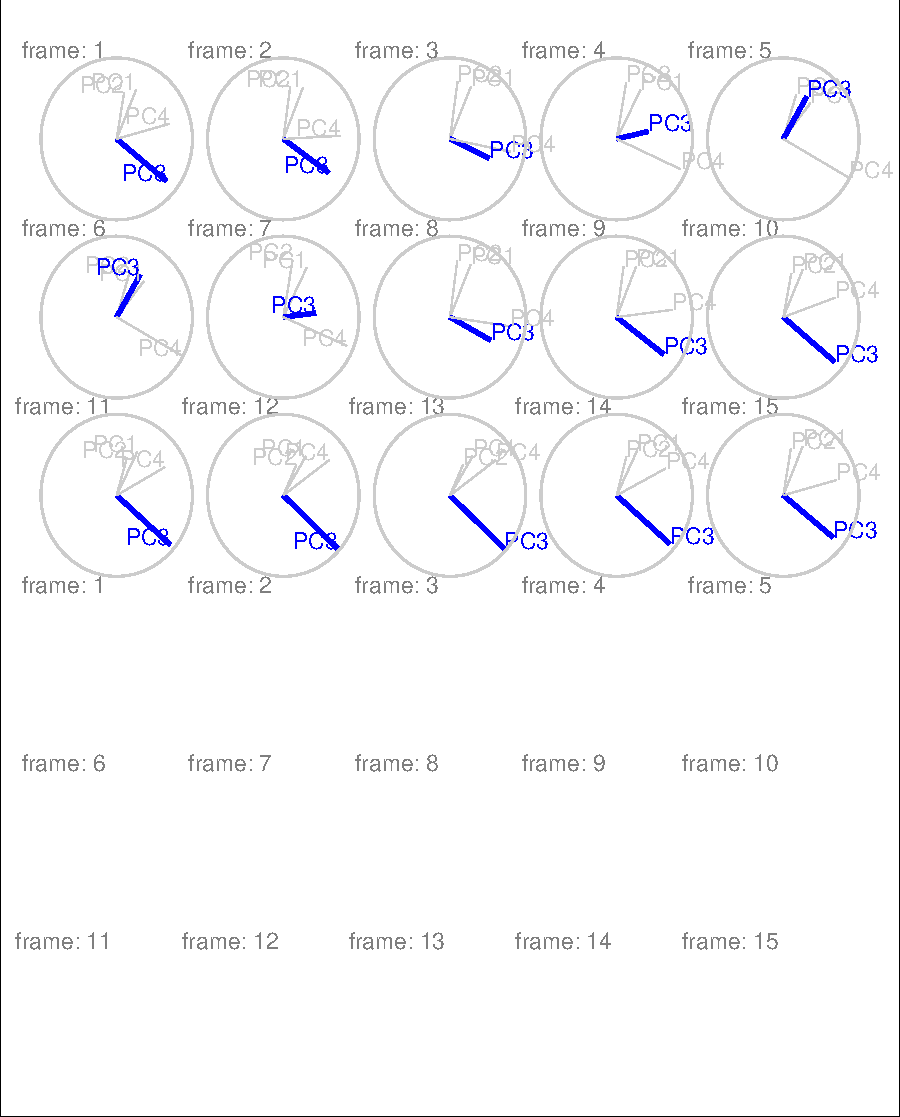
\includegraphics[width=6in,height=7.2in]{confirmation_report_ns_files/figure-latex/JetClusterGood-1} 

}

\caption{Jet cluster, a radial manual tour of PC3.
Colored by experiment type: `ATLAS7new' in green and `ATLAS7old' in
orange. When PC3 fully contributes to the projection ATLAS7new (green)
occupies unique space and several outliers are identifiable. Zeroing the
contribution from PC3 to the projection hides the outliers and indeed
all observations with ATLAS7new are contained within ATLAS7old (orange).
A dynamic version can be viewed at
\url{https://nspyrison.netlify.com/thesis/jetcluster_manualtour_pc3/}.}\label{fig:JetClusterGood}
\end{figure}









\begin{figure}

{\centering 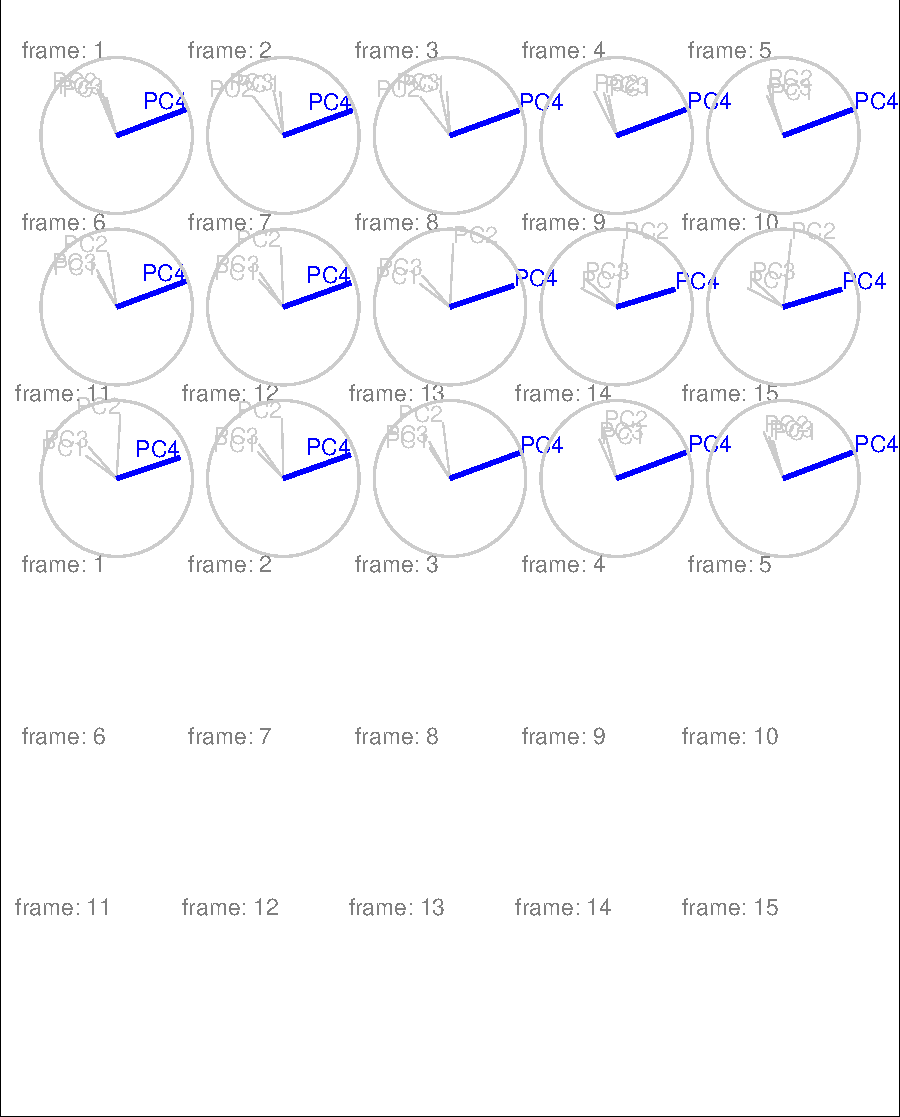
\includegraphics[width=6in,height=7.2in]{confirmation_report_ns_files/figure-latex/JetClusterBad-1} 

}

\caption{Jet cluster, a radial manual tour of PC4.
Colored by experiment type: `ATLAS7new' in green and `ATLAS7old' in
orange. This tour contains less interesting information ATLAS7new
(green) has points that are right and left of ATLAS7old, while most
points occupy the same projection space, regardless of the contribution
of PC4. A dynamic version can be viewed at
\url{https://nspyrison.netlify.com/thesis/jetcluster_manualtour_pc3/}.}\label{fig:JetClusterBad}
\end{figure}

Jet cluster manual tours manipulating each of the principal components
can be viewed from the links:
\href{https://nspyrison.netlify.com/thesis/jetcluster_manualtour_pc1/}{PC1},
\href{https://nspyrison.netlify.com/thesis/jetcluster_manualtour_pc2/}{PC2},
\href{https://nspyrison.netlify.com/thesis/jetcluster_manualtour_pc3/}{PC3},
and
\href{https://nspyrison.netlify.com/thesis/jetcluster_manualtour_pc4/}{PC4}.

\subsection{DIS cluster}\label{dis-cluster}

We perform a manual tour on this data, manipulating PC6 as depicted in
figure \ref{fig:DISclusterGood}. Looking at several frames we see that
DIS HERA data lies mostly on a plane. When PC6 has full contributions,
we see the dimuon SIDIS in purple is almost orthogonal to the DIS HERA
(green). Yet the contribution of PC6 has zeroed the dimuon SIDIS data
occupy the same space as the DIS HERA data. A dynamic version of this
manual tour can be found at:
\url{https://nspyrison.netlify.com/thesis/discluster_manualtour_pc6/}.
The page may some time to load, as the animation is several megabytes.











\begin{figure}

{\centering 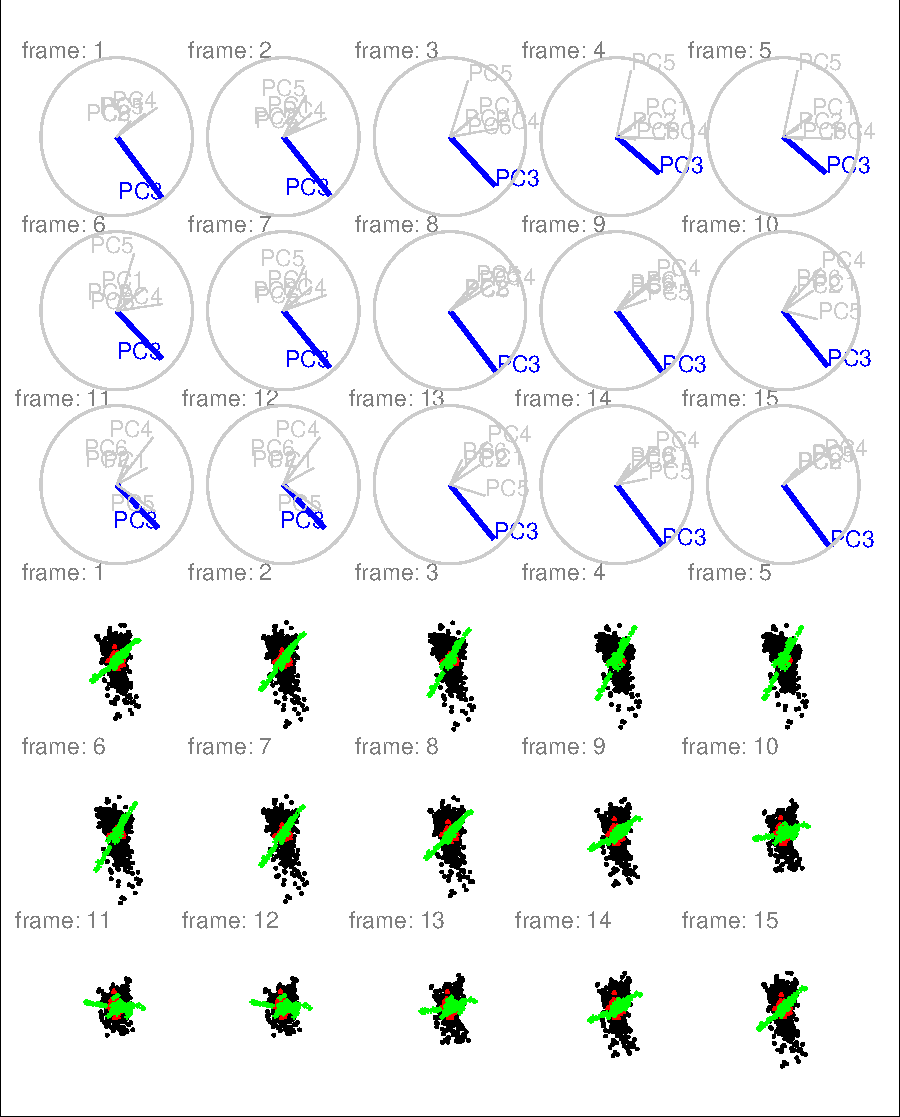
\includegraphics[width=6in,height=7.2in]{confirmation_report_ns_files/figure-latex/DISclusterGood-1} 

}

\caption{DIS cluster, a radial manual tour of PC6.
colored by experiment type: `DIS HERA1+2' in green, `dimuon SIDIS' in
purple, and `charm SIDIS' in orange. When the contribution PC 6 is large
we see that dimuon SIDIS (purple) data are nearly orthogonal to DIS HERA
(green) data. As the projection is rotated, we can also see that DIS
HERA (green) practically lies on a plane in this 6-d subspace. When the
contribution of PC6 is near zero, dimonSIDIS (purple) occupies the same
space as the DIS HERA data. A dynamic version can be viewed at
\url{https://nspyrison.netlify.com/thesis/discluster_manualtour_pc6/}.}\label{fig:DISclusterGood}
\end{figure}

The selection of the correct manip variable is important as the
manipulation spaces convey different information. For example, in figure
\ref{fig:DISclusterBad} we select PC2 as the manip variable finding it
to be less insightful than PC6.










\begin{figure}

{\centering 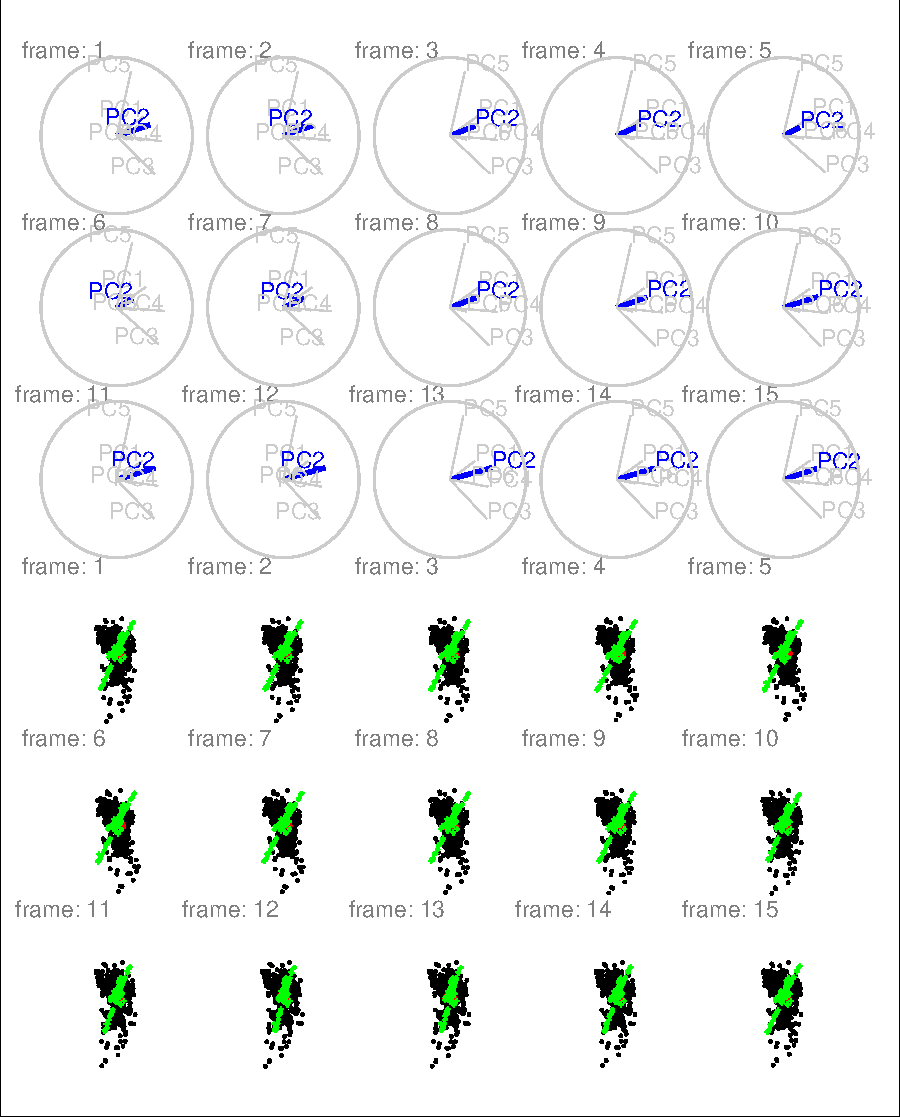
\includegraphics[width=6in,height=7.2in]{confirmation_report_ns_files/figure-latex/DISclusterBad-1} 

}

\caption{DIS cluster, a radial manual tour of PC2.
Colored by experiment type: `DIS HERA1+2' in green, `dimuon SIDIS' in
purple, and `charm SIDIS' in orange. The structure of previously
described plane of DIS HERA (green) and nearly orthogonal dimuon SIDIS
(purple) is present, however, the manipulating PC2 does not give a
head-on view of either, a less useful manual tour than that of PC6. A
dynamic version can be viewed at
\url{https://nspyrison.netlify.com/thesis/discluster_manualtour_pc2/}.}\label{fig:DISclusterBad}
\end{figure}

DIS cluster manual tours manipulating each of the principal components
can be viewed from the links:
\href{https://nspyrison.netlify.com/thesis/discluster_manualtour_pc1/}{PC1},
\href{https://nspyrison.netlify.com/thesis/discluster_manualtour_pc2/}{PC2},
\href{https://nspyrison.netlify.com/thesis/discluster_manualtour_pc3/}{PC3},
\href{https://nspyrison.netlify.com/thesis/discluster_manualtour_pc4/}{PC4},
\href{https://nspyrison.netlify.com/thesis/discluster_manualtour_pc5/}{PC5},
and
\href{https://nspyrison.netlify.com/thesis/discluster_manualtour_pc6/}{PC6}.

\section{Source code and usage}\label{source-code-and-usage}

This article was created in \texttt{R} \autocite{r_core_team_r:_2018},
using \texttt{bookdown} \autocite{xie_bookdown:_2016} and
\texttt{rmarkdown} \autocite{xie_r_2018}, with code generating the
examples inline. The source files can be found at
\href{https://github.com/nspyrison/confirmation/}{github.com/nspyrison/confirmation/}.

The source code for the \texttt{spinifex} package can be found at
\href{https://github.com/nspyrison/spinifex/}{github.com/nspyrison/spinifex/}.
To install the package in R, run:

\begin{Shaded}
\begin{Highlighting}[]
\CommentTok{# install.package("devtools")}
\NormalTok{devtools}\OperatorTok{::}\KeywordTok{install_github}\NormalTok{(}\StringTok{"nspyrison/spinifex"}\NormalTok{)}
\end{Highlighting}
\end{Shaded}

\section{Discussion}\label{sec:discussion}

This research has modified the algorithm producing manual tours in
extends animations of tours to other graphics packages. Tour paths
generated in \texttt{tourr} can also be viewed using these frameworks.

Future research on the algorithm would include extending it for use in
3D projections. This would allow for projections in immersive virtual
reality, which may allow for a better perception of structure and enable
function visualization. The \texttt{tourr} package provides many other
geometric displays with the \texttt{tourr::display\_*()} family. These
other geoms should be integrated into the \texttt{ggplot2} framework for
display on \texttt{plotly} and \texttt{gganimate}.

The Givens rotations and Householder reflections as outlined in
\textcite{buja_computational_2005} could also be added. Currently,
Gram-Schmidt is the only form of frame interpolation used. In a Givens
rotation, the \(x\) and \(y\) components (for example
\(\theta~= 0,~pi/2\)) of the in-plane rotation are calculated separately
and would be applied sequentially to produce the radial rotation.
Householder reflections define reflection axes to project points on to
the axes and generate rotations.

The development of a dynamic graphical user interface, perhaps with the
use of a \texttt{shiny} app, would allow analysts to rapidly try manual
tours with a more intuitive interaction than the command line. The user
could easily switch between variables to control, adjust the step size
to make smoother rotation sequences, or save any state to continue to
explore the contributions of other variables. The \texttt{animation}
package \textcite{xie_animation:_2018} could be implemented for another
graphics framework. However, \texttt{animation} builds from base graphs
while \texttt{spinifex} current utilizes \texttt{ggplot2} graphics.

\printbibliography[heading=bibintoc]



\end{document}
